\section{Geometrija na ravnini in v prostoru}

\begin{frame}
    \sectionpage
\end{frame}

\begin{frame}
    \tableofcontents[currentsection, hideothersubsections]
\end{frame}

    \subsection{Osnovni geometrijski pojmi}

        \begin{frame}
            \frametitle{Osnovni geometrijski pojmi}
        \end{frame}

    \subsection{Kot}

        \begin{frame}
            \frametitle{Kot}
        \end{frame}

    \subsection{Konstrukcije matematičnih objektov}

        \begin{frame}
            \frametitle{Konstrukcije matematičnih objektov}
        \end{frame}

    \subsection{Preslikave na ravnini}

        \begin{frame}
            \frametitle{Preslikave na ravnini}

            \large\textbf{Pravokotna projekcija}
            ~\\

            \normalsize
            \begin{columns}
                \column{0.62\textwidth}
                    \begin{alertblock}{}
                        Dani sta točka $T$ in premica $p$. Naj bo $q$ tista pravokotnica na premico $p$, ki poteka skozi točko $T$. 
                        Presečišče $T'$ premice $q$ s premico $p$ imenujemo \textbf{pravokotna projekcija} točke $T$ na premico $p$. 
                        Točka $T'$ je točki $T$ najbližja točka premice $p$. \\
                    \end{alertblock}
                    % ~\\
                    \begin{alertblock}{}
                        \textbf{Razdalja} točke $T$ od premice $p$ je: \\ $\quad \quad \quad \quad d(T,p)=d(T,T')=\left\lvert TT'\right\rvert$. \\
                    \end{alertblock} ~\\

                \column{0.35\textwidth}            
                    \begin{figure}
                    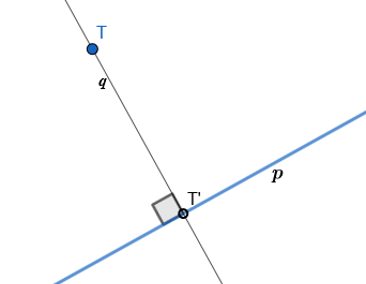
\includegraphics[scale=0.5]{Slike in skice/Pravokotna_projekcija.png}
                    \end{figure}
            \end{columns}

            Pravokotna projekcija daljice $AB$ na premico je daljica $A'B'$, katere krajišči sta pravokotni projekciji točko $A$ in $B$.

            
        \end{frame}

        \begin{frame}
            \large\textbf{Toge preslikave}
            ~\\
            \normalsize

            \begin{alertblock}{}
                \textbf{Toga preslikava} (izometrija) je preslikava v ravnini, ki ohranja razdalje.
                \begin{align*}
                    \tau:~ &A \mapsto A' \\ 
                    \tau:~ &B \mapsto B' \\ 
                    d(A,B)&=d(A',B')
                \end{align*}
            \end{alertblock}

            Med toge preslikave spadajo:
                \begin{itemize}
                    \item \textbf{vzporedni premiki};
                    \item \textbf{zrcaljenje preko premice};
                    \item \textbf{zrcaljenje preko točke};
                    \item \textbf{rotacija okoli točke}.
                \end{itemize}

            Če kombiniramo več togih premikov, je dobljena preslikava spet togi premik.

        \end{frame}

        \begin{frame}
            \large\textbf{Vzporedni premik/translacija}
            ~\\
            ~\\
            \normalsize
            \textbf{Vzporedni premik} ali \textbf{translacija} za dano usmerjeno daljico (vektor) $\overrightarrow{AB}$ preslika točko $T$ v tako točko $T'$, da sta daljici $TT'$ in $AB$ enako dolgi, vzporedni in enako usmerjeni (vektorja $\overrightarrow{TT'}$ in $\overrightarrow{AB}$ sta enaka). \\
            
            \begin{figure}
                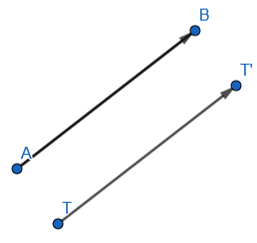
\includegraphics[scale=0.5]{Slike in skice/Vzporedni_premik_tocke.png}
                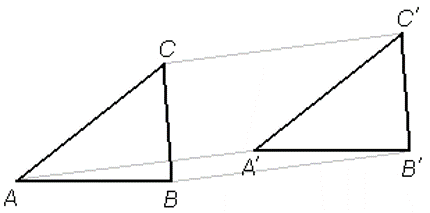
\includegraphics[scale=0.5]{Slike in skice/Vzporedni_premik_trikotnika.png}
            \end{figure}

            Vzporedni premik ohranja orientacijo likov, daljice preslika v enako dolge vzporedne daljice, ohranja velikost kotov, like preslika v skladne like, nima negibnih točk za $\overrightarrow{AB}\neq \overrightarrow{0}$.

        \end{frame}


        \begin{frame}
            \large\textbf{Rotacija/vrtenje okoli točke}
            ~\\
            ~\\
            \normalsize
            \textbf{Vrtenje} ali \textbf{zasuk} oziroma \textbf{rotacija} za kot $\alpha$ okrog točke $O$ preslika točko $T$ v točko $T'$, da velja: $\left\lvert OT\right\rvert = \left\lvert OT'\right\rvert$  in $\angle TOT' = \alpha$.


            \begin{figure}
                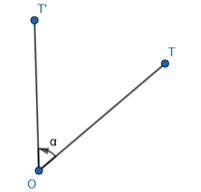
\includegraphics[scale=0.6]{Slike in skice/Rotacija tocke_okoli_tocke.png}
                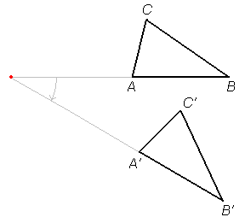
\includegraphics[scale=0.6]{Slike in skice/Rotacija_lika_okoli_tocke.png}
            \end{figure}

            Vrtenje okoli točke preslika daljice v enako dolge daljice, ohranja velikosti kotov in orientacijo likov, like preslika v skladne like, premice pa ne preslika v vzporedne premice. 

        \end{frame}

        % \begin{frame}
            
        %     Če smo kot  odmerili v smeri, ki je nasprotna smeri vrtenja urinega kazalca, smo točko $T$ zavrteli v \textbf{pozitivni smeri} za kot $\alpha$, sicer pa v \textbf{negativni smeri}. 
        %     Namesto smeri vrtenja lahko usmerimo kot: vrtenju v pozitivni smeri ustreza \textbf{pozitivni kot}, vrtenju v negativni smeri pa \textbf{negativni kot}. \\
        %     ~\\

        %     Vrtenje okoli točke preslika daljice v enako dolge daljice, ohranja velikosti kotov in orientacijo likov, like preslika v skladne like, premice pa ne preslika v vzporedne premice. 

        % \end{frame}


        \begin{frame}
            \large\textbf{Zrcaljenje preko premice}
            ~\\
            ~\\
            \normalsize
            \textbf{Zrcaljenje čez premico} $p$ preslika točko $T$ v tako točko $T'$, da premica $p$ pod pravim kotom razpolavlja daljico $TT'$.
            
            \begin{figure}
                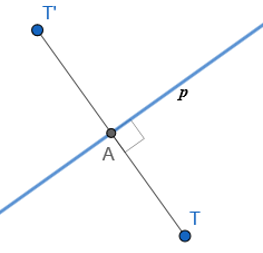
\includegraphics[scale=0.5]{Slike in skice/Zrcaljenje_tocke_cez_premico.png}
                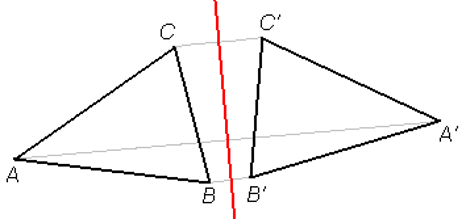
\includegraphics[scale=0.5]{Slike in skice/Zrcaljenje_lika_cez_premico.png}
            \end{figure}

            Zrcaljenje čez premico daljice preslika v enako dolge daljice, ohranja velikost kotov, ne ohranja orientacije likov, like preslika v skladne like, premic ne preslika v vzporedne premice.

        \end{frame}

        
        \begin{frame}
            \large\textbf{Zrcaljenje preko točke}
            ~\\
            ~\\
            \normalsize
            \textbf{Zrcaljenje čez točko} $O$ preslika točko $T$ v tako točko $T'$, da je $O$ razpolovišče daljice $TT'$. Ta preslikava je enaka vrtenju okrog točke za $180^\circ$.

            \begin{figure}
                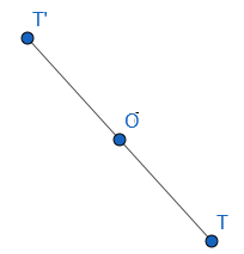
\includegraphics[scale=0.5]{Slike in skice/Zrcaljenje_tocke_cez_tocko.png}
                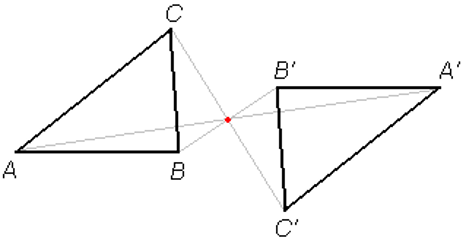
\includegraphics[scale=0.5]{Slike in skice/Zrcaljenje_lika_cez_tocko.png}
            \end{figure}

            Zrcaljenje čez točko daljice preslika v enako dolge daljice, ohranja velikosti kotov in orientacijo likov, like preslika v skladne like, premice preslika v vzporedne premice.

        \end{frame}



        \begin{frame}
            \large\textbf{Simetrija}
            ~\\
            ~\\
            \normalsize
            \begin{columns}
                \column{0.65\textwidth}
                Množica točk $\mathcal{M}$ je \textbf{simetrična/somerna glede na premico} $p$, če se pri zrcaljenju čez premico $p$ preslika sama vase. Premico $p$ imenujemo \textbf{simetrala}, \textbf{somernica}, \textbf{simetrijska os} množice $\mathcal{M}$. \\
                 ~\\      
                 ~\\      
                Množica točk $\mathcal{M}$ je \textbf{središčno simetrična/somerna glede na točko} $T$, če se pri zrcaljenju čez točko $T$ preslika sama vase. Točko $T$ imenujemo \textbf{center simetrije} množice $\mathcal{M}$. 
                \column{0.32\textwidth}
                \begin{figure}
                    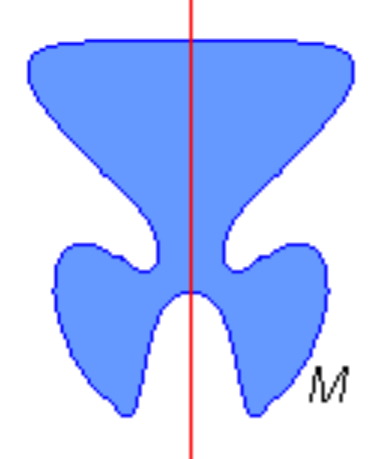
\includegraphics[scale=0.25]{Slike in skice/Simetrija glede na premico.png}

                    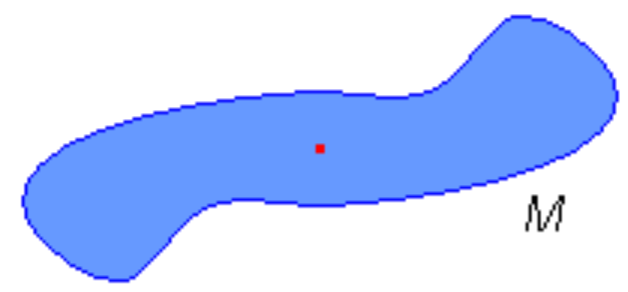
\includegraphics[scale=0.25]{Slike in skice/Simetrija glede na točko.png}
                \end{figure}
            \end{columns}


        \end{frame}

    \subsection{Trikotnik}

        \begin{frame}
            \frametitle{Trikotnik}

            \begin{alertblock}{}
                \textbf{Trikotnik} je lik/množica točk v ravnini, omejena s tremi daljicami -- \textbf{stranice} ($a, b, c$), ki povezujejo tri nekolinearne točke ($A, B, C$) v ravnini. Te točke imenujemo \textbf{oglišča} trikotnika.
            \end{alertblock}
            
            \begin{figure}
                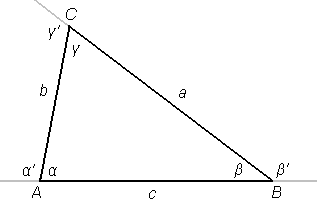
\includegraphics[scale=0.7]{Slike in skice/Trikotnik.png}    
            \end{figure}

            V trikotniku $\triangle ABC$  so $\alpha, \beta$ in $\gamma$ \textbf{notranji koti}, njihovi sokoti $\alpha', \beta'$ in $\gamma'$ pa so \textbf{zunanji koti}. 
            
        \end{frame}

        \begin{frame}
            
            \begin{alertblock}{}
                Vsota notranjih kotov trikotnika je $180^\circ$: $$\alpha+\beta+\gamma=180^\circ.$$ 
            \end{alertblock}

            \begin{alertblock}{}
                Zunanji kot trikotnika je enak vsoti notranjih nepriležnih kotov: 
                \begin{align*}
                    \alpha' &= \beta+\gamma \\
                    \beta' &= \alpha+\gamma \\
                    \gamma' &= \alpha+\beta
                \end{align*}
            \end{alertblock}

            \begin{alertblock}{}
                Vsota zunanjih kotov trikotnika je $360^\circ$: $$\alpha'+\beta'+\gamma'=360^\circ.$$ 
            \end{alertblock}

        \end{frame}


        \begin{frame}
            
            \begin{alertblock}{}
                Nasproti daljše stranice trikotnika leži večji notranji kot, nasproti krajše stranice pa manjši notranji kot trikotnika.
                $$a>b \Leftrightarrow \alpha > \beta$$
            \end{alertblock}

            \begin{alertblock}{Trikotniška neenakost}
                Vsaka stranica trikotnika je krajša od vsote dolžin drugih dveh stranic.
                \begin{align*}
                    a &< b + c \\
                    b &< a + c \\
                    c &< a + b
                \end{align*}
            \end{alertblock}

            \begin{alertblock}{}
                Vsaka stranica trikotnika je daljša od absolutne vrednosti razlike dolžin drugih dveh stranic.
            \end{alertblock}

        \end{frame}


        \begin{frame}

            \begin{alertblock}{}
                \textbf{Višina} na stranico trikotnika je daljica, ki povezuje nosilko te stranice z nasprotnim ogliščem in je pravokotna na to nosilko. 
                Njena dolžina je razdalja oglišča od nasprotne stranice.
            \end{alertblock}

            \begin{figure}
                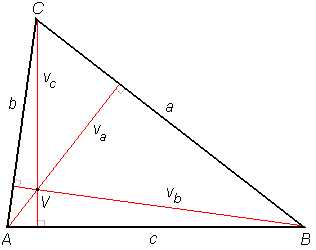
\includegraphics[scale=0.5]{Slike in skice/Visina_in_visinska_tocka.png}
            \end{figure}

            \begin{alertblock}{}
                Nosilke vseh treh višin na stranice trikotnika se sekajo v eni točki, ki jo imenujemo \textbf{višinska točka} ali \textbf{ortocenter}. Standardna oznaka: $V$ ali $H$.
            \end{alertblock}

        \end{frame}


        \begin{frame}

            \begin{alertblock}{}
                \textbf{Težiščnica} na stranico trikotnika je daljica, ki povezuje razpolovišče te stranice z nasprotnim ogliščem. 
            \end{alertblock}

            \begin{figure}
                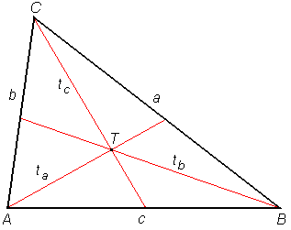
\includegraphics[scale=0.5]{Slike in skice/Teziscnice_in_tezisce.png}
            \end{figure}

            \begin{alertblock}{}
                Vse tri trikotnikove težiščnice se sekajo v eni točki -- \textbf{težišču} ali \textbf{baricentru} trikotnika. 
                Težišče deli težiščnico v razmerju $1:2$.
            \end{alertblock}

        \end{frame}


        \begin{frame}

            \begin{alertblock}{}
                Simetrale vseh treh stranic trikotnika se sekajo v eni točki. Ta točka je \textbf{središče trikotniku očrtane krožnice}. 
            \end{alertblock}

            \begin{figure}
                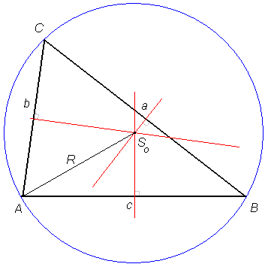
\includegraphics[scale=0.55]{Slike in skice/Trikotniku_ocrtana_kroznica.png}
            \end{figure}

            Očrtana krožnica poteka skozi vsa tri oglišča trikotnika. Vse tri stranice trikotnika so tetive te krožnice.

        \end{frame}


        \begin{frame}

            \begin{alertblock}{}
                Simetrale notranjih kotov trikotnika se sekajo v eni točki. Ta točka je \textbf{središče trikotniku včrtane krožnice}.
            \end{alertblock}

            \begin{figure}
                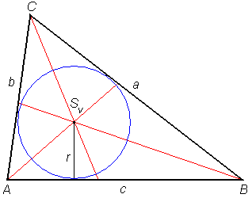
\includegraphics[scale=0.65]{Slike in skice/Trikotniku_vcrtana_kroznica.png}
            \end{figure}
            
            Včrtana krožnica ima vse tri stranice trikotnika za tangente.

        \end{frame}


        \begin{frame}

            \begin{alertblock}{}
                Težišče, središče trikotniku očrtane kroznice, središče trikotniku včrtane krožnice in višinska točka so \textbf{znamenite točke trikotnika}.

            \end{alertblock}

            \begin{alertblock}{}
                Višinska točka, središče očrtane krožnice in težišče so vedno kolinearne. Premico, ki jih povezuje, imenujemo \textbf{Eulerjeva premica}.
            \end{alertblock}

            \begin{figure}
                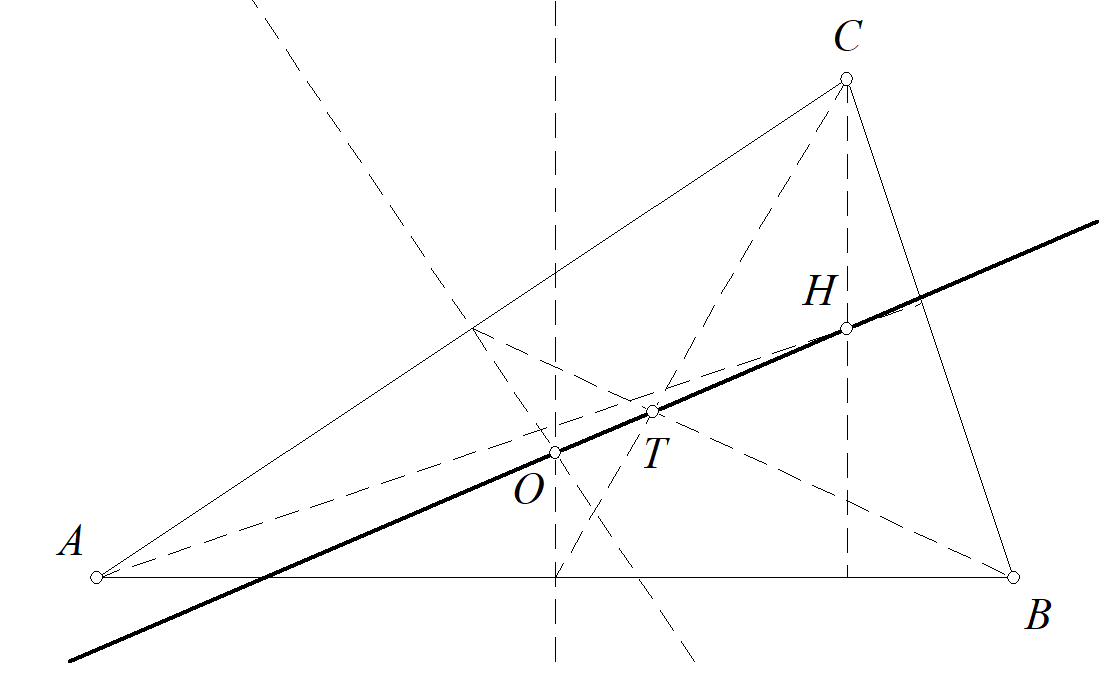
\includegraphics[scale=0.23]{Slike in skice/Eulerjeva_premica.png}
            \end{figure}
            

        \end{frame}

    \subsection{Krog}

        \begin{frame}
            \frametitle{Krog}
        \end{frame}

    \subsection{Štirikotnik}

        \begin{frame}
            \frametitle{Štirikotnik}
        \end{frame}

    \subsection{Večkotnik}

        \begin{frame}
            \frametitle{Večkotnik}
        \end{frame}

    \subsection{Podobnost}

        \begin{frame}
            \frametitle{Podobnost}
        \end{frame}

    \subsection{Podobnost v pravokotnem trikotniku}
        
        \begin{frame}
            \frametitle{Podobnost v pravokotnem trikotniku}
        \end{frame}

    \subsection{Kotne funkcije kotov, velikih od $0^\circ$ do $90^\circ$}
        
        \begin{frame}
            \frametitle{Kotne funkcije kotov, velikih od $0^\circ$ do $90^\circ$}
        \end{frame}
        
    \subsection{Kotne funkcije kotov, velikih od $0^\circ$ do $160^\circ$}
        
        \begin{frame}
            \frametitle{Kotne funkcije kotov, velikih od $0^\circ$ do $360^\circ$}
        \end{frame}
